\documentclass[addpoints]{exam}

%\printanswers
\noprintanswers

\usepackage{amsmath,bigstrut,minted,url,graphicx,tikz,tikz-qtree}

\pagestyle{headandfoot}
\runningheadrule
\firstpageheader{}{}{Page \thepage\ of \numpages}
\runningheader{CS 321}{Sample Problems}{Page \thepage\ of \numpages}
\firstpagefooter{}{}{}
\runningfooter{}{}{}
              
\begin{document}

\begin{center}
{\Large \textbf{
    Ozyegin University\\
    CS 321 Programming Languages\\
    Sample Problems on Interpretation
}}
\end{center}

\begin{questions}
  \question
  (From PLC, Exercise 1.1)
  Given the definition of the simple ArithLang below,
  extend this language with conditional expressions (i.e. ``if'')
  corresponding to Java's expression \texttt{$e_1$ ? $e_2$ : $e_3$},
  or OCaml's \texttt{if $e_1$ then $e_2$ else $e_3$}.
  Evaluation of a conditional expression should evaluate $e_1$ first.
  If it yields a non-zero value, evaluate $e_2$, otherwise evaluate $e_3$.
  
  \inputminted{ocaml}{arith.ml}

  \begin{solutionbox}{9cm}
    Here is the diff:
    \inputminted{diff}{arith_if_diff.txt}
  \end{solutionbox}


  \newpage
  \question
  (From PLC, Exercise 1.1)
  Extend ArithLang to handle three additional operators:
  ``max'', ``min'', and ``=''.
  Like the existing binary operators,
  they take two argument expressions.
  The equals operator should return 1 when true and 0 when false.

  \begin{solutionbox}{14cm}
    Here is the diff:
    \inputminted{diff}{arith_minmaxeq_diff.txt}
  \end{solutionbox}

  
  \question
  Write the representation of the following ArithLang expressions
  using the \texttt{exp} data type.
  \begin{parts}
    \part \mintinline{ocaml}{v * 5 - k + 6}
    \begin{solutionbox}{1cm}
      \mintinline{ocaml}{Add(Subt(Mult(Var "v", CstI 5), Var "k"), CstI 6)}
    \end{solutionbox}
    
    \part \mintinline{ocaml}{x + y + z + p}
    \begin{solutionbox}{1cm}
      \mintinline{ocaml}{Add(Add(Add(Var "x", Var "y"), Var "z"), Var "p")}
    \end{solutionbox}
    
    \part \mintinline{ocaml}{5 - (y - 3) * (g + 1)}
    \begin{solutionbox}{1cm}
      \mintinline{ocaml}{Subt(CstI 5, Mult(Subt(Var "y", CstI 3), Add(Var "g", CstI 1)))}
    \end{solutionbox}  

    \part
    \begin{minted}{ocaml}
    let x =
      let a = 5
      in let b = 8
         in a + b
    in x * (let y = x + 2 in y)
    \end{minted}
    \begin{solutionbox}{4cm}
      \begin{minted}{ocaml}
        LetIn("x",
              LetIn("a", CstI 5,
                    LetIn("b", CstI 8,
                          Add(Var "a", Var "b"))),
              Mult(Var "x",
                   LetIn("y", Add(Var "x", CstI 2),
                         Var "y"))) 
      \end{minted}
    \end{solutionbox}  
\end{parts}


  \question
  Write an OCaml function named \texttt{simplify}
  that takes an \texttt{exp} and returns its simplified form
  based on the rules below:

  {
    \begin{center}
    \begin{tabular}{c}\hline
      $0+e \to e$\\
      $e+0 \to e$\\
      $e-0 \to e$\\
      $1\times e \to e$\\
      $e\times 1 \to e$\\
      $0\times e \to 0$\\
      $e\times 0 \to 0$\\
      $e-e \to 0$\\\hline
    \end{tabular}
    \end{center}
  }

  Remark: This problem is harder than it seems, because
  simplification of expressions may enable other simplifications,
  and I want to you to handle those cases, too.   
  See the test cases.

  \begin{minted}{ocaml}
    # simplify (Mult(CstI 1,
                     Mult(Add(Add(CstI 1,
                                  Subt(Var "x", Var "x")),
                              Add(CstI 4, CstI 6)),
                          CstI 1)));;
    - : exp = Add(CstI 1, Add(CstI 4, CstI 6))
    
    # simplify (Subt(CstI 0, Mult(Add(Var "x", CstI 0), CstI 0)));;
    - : exp = CstI 0
    
    # simplify (LetIn("a", CstI 4,
                      Subt(CstI 0,
                           Mult(Add(Var "x", CstI 0),
                                CstI 0))));;
    - : exp = LetIn("a", CstI 4, CstI 0)

    # simplify (Subt(Add(CstI 7, CstI 0),
                     Mult(Add(Var "x", CstI 0), CstI 0)));;
    - : exp = CstI 7

    # simplify (Div(Subt(CstI 0,
                         Mult(Add(Var "x", CstI 0), CstI 0)),
                    CstI 7));;
    - : exp = Div(CstI 0, CstI 7)
  \end{minted}

  \begin{solutionbox}{11cm}
    \inputminted{ocaml}{simplify.ml}
  \end{solutionbox}

  \question
  Is the grammar shown below ambiguous?
  If yes, give me an input that at least two different
  parse trees, and show those trees.
  If no, prove it.

  \begin{minted}{ocaml}
    main ::= exp EOF
    exp  ::= INT
           | NAME
           | exp PLUS exp
           | exp STAR exp
           | LET NAME EQ exp IN exp
           | IF exp THEN exp ELSE exp
  \end{minted}

  \begin{solutionbox}{12cm}
    It is ambiguous. Here is an input:
    \mintinline{ocaml}{let x = 5 in x + 9}.

    \Tree[.main
      [.exp
        LET
        {NAME(``x'')}
        EQ
        [.exp {INT(5)} ]
        IN
        [.exp
          [.exp {NAME(``x'')} ]
          PLUS
          [.exp {INT(9)} ]
        ]
      ]
      EOF
    ]
    
    And the second tree is
        
    \Tree[.main
      [.exp
        [.exp
          LET
          {NAME(``x'')}
          EQ
          [.exp {INT(5)} ]
          IN
          [.exp {NAME(``x'')} ]
        ]
        PLUS
        [.exp {INT(9)} ]
      ]
      EOF
    ]
  \end{solutionbox}

  \question
  \begin{minted}{ocaml}
    main ::= exp EOF
    exp  ::= INT
           | NAME
           | exp SLASH exp
           | exp PLUS exp
           | LET NAME EQ exp IN exp
           | IF exp THEN exp ELSE exp
  \end{minted}
  Based on the grammar given above,
  show two different parse trees for the following inputs.
  For each, also state whether the ambiguity is related to
  \textbf{precedence} or \textbf{associativity}.
  \begin{parts}
    \part \mintinline{ocaml}{9 + 5 + 2}
    \begin{solutionbox}{6.5cm}
      This is related to associativity.
      Does the ``+'' sign associate to the left or to the right? That's the problem.
      If ``+'' associates to the right, we would get the tree on the left;
      if ``+'' associates to the left, we would get the tree on the right.

      {\small
      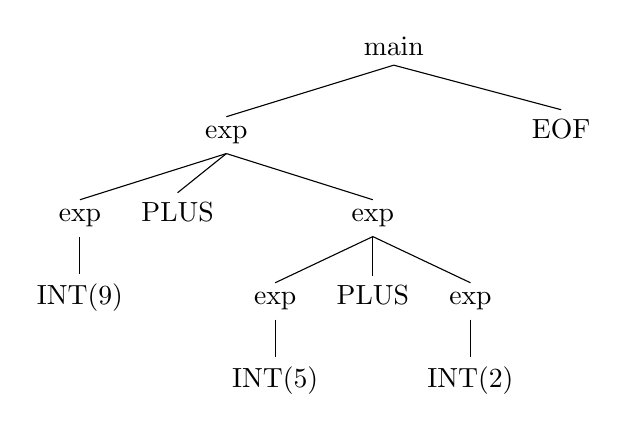
\begin{tikzpicture}[sibling distance=0pt]
        \Tree[.main
        [.exp
          [.exp INT\\(9) ]
          PLUS
          [.exp
            [.exp {INT(5)} ]
            PLUS
            [.exp {INT(2)} ]
          ]
        ]
        EOF
      ]
      \end{tikzpicture}
      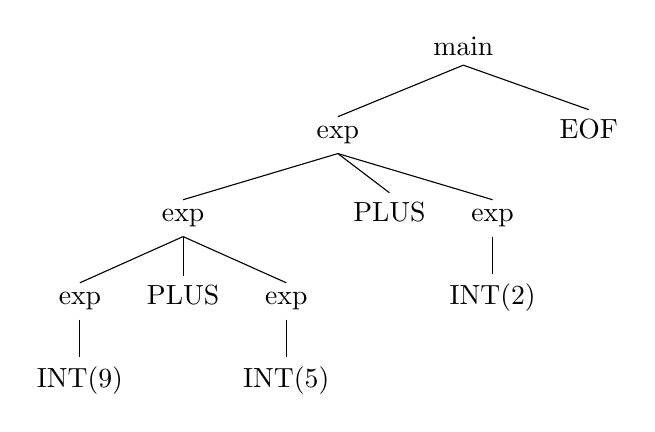
\begin{tikzpicture}
      \Tree[.main
        [.exp
          [.exp
            [.exp {INT(9)} ]
            PLUS
            [.exp {INT(5)} ]
          ]
          PLUS
          [.exp {INT(2)} ]
        ]
        EOF
      ]
      \end{tikzpicture}
      }
    \end{solutionbox}
    
    \part \mintinline{ocaml}{9 + 5 / 2}
    \begin{solutionbox}{7cm}
      This is related to precedence.
      Which operator has higher precedence, ``/'' or ``+''?
      That is, who wins the fight over the ownership of ``5''?
      That's the problem.
      If ``/'' has higher precedence, we would get the tree on the left;
      if ``+'' has higher precedence, we would get the tree on the right.

      {\small
      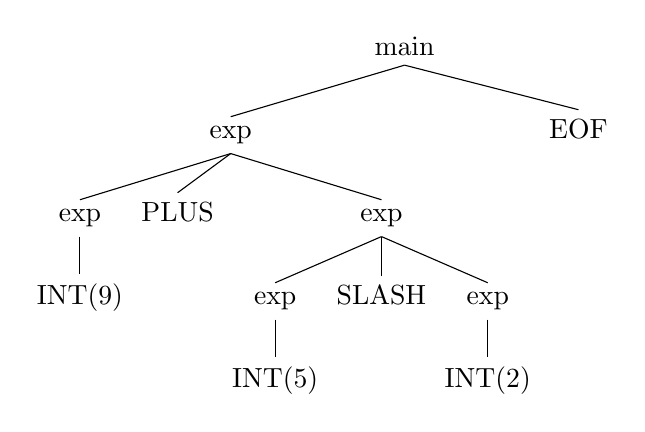
\begin{tikzpicture}[sibling distance=0pt]
        \Tree[.main
        [.exp
          [.exp INT\\(9) ]
          PLUS
          [.exp
            [.exp {INT(5)} ]
            SLASH
            [.exp {INT(2)} ]
          ]
        ]
        EOF
      ]
      \end{tikzpicture}
      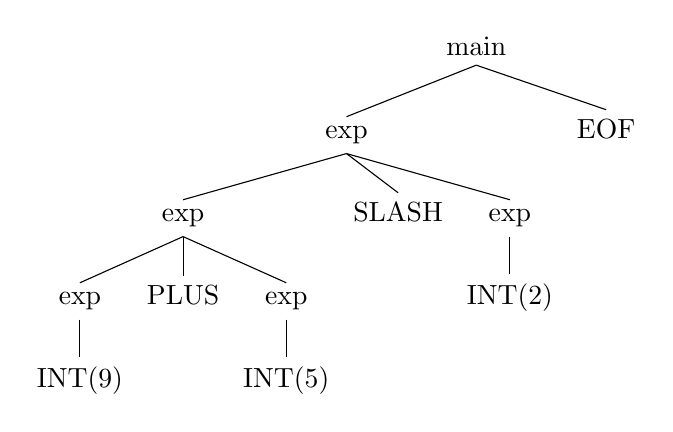
\begin{tikzpicture}
      \Tree[.main
        [.exp
          [.exp
            [.exp {INT(9)} ]
            PLUS
            [.exp {INT(5)} ]
          ]
          SLASH
          [.exp {INT(2)} ]
        ]
        EOF
      ]
      \end{tikzpicture}
      }
    \end{solutionbox}
  \end{parts}
  
  \question
  The following is an ambiguous grammar. 
  Non-terminals in the notation are written using
  lowercase letters;
  terminals are all in capital letters.
  Give a term that has at least two different parse trees
  in this grammar.
  Show those two trees.
  
  \begin{verbatim}
    expr ::= expr PLUS atom
           | IF expr THEN expr ELSE expr
           | BOOL

    atom ::= NAME
  \end{verbatim}

  \begin{solutionbox}{8.5cm}
    Consider ``if true then true else true + x''.

    {\small
      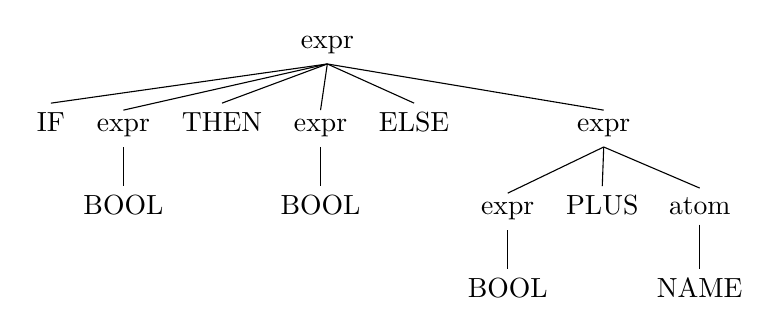
\begin{tikzpicture}[sibling distance=0pt]
        \Tree[.expr
          IF
          [.expr BOOL ]
          THEN
          [.expr BOOL ]
          ELSE
          [.expr
            [.expr BOOL ]
            PLUS
            [.atom NAME ]
          ]
        ]
      \end{tikzpicture}

      \hrule
      
      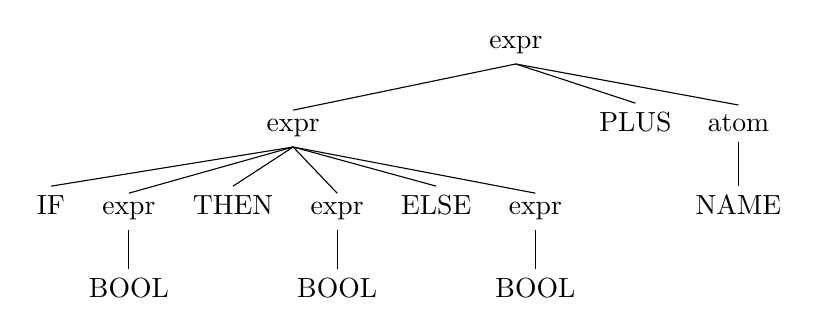
\begin{tikzpicture}
        \Tree[.expr
          [.expr
            IF
            [.expr BOOL ]
            THEN
            [.expr BOOL ]
            ELSE
            [.expr BOOL ]
          ]
          PLUS
          [.atom NAME ]
        ]
      \end{tikzpicture}
    }
  \end{solutionbox}

  
  \question
  Write a lexer that recognizes all character sequences
  consisting of 
  $a$ and $b$ where two $a$'s are always separated by at least one $b$.
  For instance, these four strings are legal: $b$, $a$, $ba$, $ababbbaba$;
  but these two strings are illegal: $aa$, $babaa$.
  Your lexer should take a list of chars, and return
  true if the input is legal, otherwise return false.

  \begin{solutionbox}{3.5cm}
    \begin{minted}{ocaml}
      let rec lexer chars =
        match chars with
        | [] -> true
        | 'a'::'a'::rest -> false
        | _::rest -> lexer rest      
    \end{minted}    
  \end{solutionbox}


  \begin{framed}
    The questions below are based on Deve 1.0, given at
    \url{https://github.com/aktemur/cs321/tree/master/Deve-1.0}.
    The code is also shown below:
  \end{framed}

  \textbf{EVALUATOR:}\\
  \inputminted{ocaml}{../../Deve-1.0/deve.ml}

  \textbf{LEXER:}\\
  \inputminted{ocaml}{../../Deve-1.0/lexer.ml}

  \textbf{PARSER:}\\
  \inputminted{ocaml}{../../Deve-1.0/parser.ml}

  
  
  \question
  Extend the Deve language interpreter to handle parenthesized expressions
  such as \texttt{(3 + 4) * 5}.

  \begin{solution}
    We need to first modify the lexer to recognize parentheses.
    For this, we will also add two more tokens:
    
    \begin{minted}{ocaml}
      type token = INT of int
                 | ...
                 | LPAR | RPAR

      let rec tokenize chars =
        match chars with
        | ...
        | '('::rest -> LPAR::(tokenize rest)
        | ')'::rest -> RPAR::(tokenize rest)
        | ...
    \end{minted}

    Now we have to update the parser.
    Because a parenthesized expression is
    ``closed'' on both sides with tokens,
    no ambiguity issues arise. For the same reason,
    a parenthesized expression is just like an ``atomic''
    expression; it should be located at the highest level of precedence.
    So, we have:

    \begin{minted}{ocaml}
and parseLevel4Exp tokens =
  match tokens with
  | ...
  | LPAR::rest ->
     let (e, tokens1) = parseExp rest in
     let rest2 = consume RPAR tokens1 in
     (e, rest2)
    \end{minted}

    A parenthesized expression is just for grouping an expression;
    we simply return the \texttt{exp} we parse between parentheses.
    No new AST constructor is created.
  \end{solution}
  
  \question
  Instead of having a separate AST constructor for
  each binary operator
  (e.g. \texttt{Add}, \texttt{Subt}, etc.),
  use a single constructor named \texttt{Binary}
  to handle any binary operator.
  For this, change the definition of the
  \texttt{exp} data type.
  In a \texttt{Binary},
  in addition to the left and the right operands,
  keep the operator as a string.
  
  E.g. \texttt{Add($e_1$, $e_2$)} becomes
  \texttt{Binary("+", $e_1$, $e_2$)};\\
  \texttt{Mult($e_1$, $e_2$)} becomes
  \texttt{Binary("*", $e_1$, $e_2$)};\\
  \texttt{Subt($e_1$, $e_2$)} becomes
  \texttt{Binary("-", $e_1$, $e_2$)}.
  
  \begin{solution}
    Here is the new definition for \texttt{exp}:
    \begin{minted}{ocaml}
      type exp = CstI of int
         | CstB of bool
         | Var of string
         | Binary of string * exp * exp
         | LetIn of string * exp * exp
         | If of exp * exp * exp
    \end{minted}

    Update the \texttt{eval} function as follows:

    \begin{minted}{ocaml}
    let rec eval e env =
      match e with
      | ...
      | Binary(op, e1, e2)  ->
         let i1 = eval e1 env in
         let i2 = eval e2 env in
         (match op with
          | "+" -> i1 + i2
          | "-" -> i1 - i2
          | "*" -> i1 * i2
          | "/" -> i1 / i2
          | ...
         )
    \end{minted}

    You will also need to modify the parser
    to return AST's according to this new definition:

    {\small
    \begin{minted}{ocaml}
...
and parseLevel2Exp tokens =
  let rec helper tokens e1 =
    match tokens with
    | PLUS::tok::rest ->
       (match tok with
        | LET -> let (e2, tokens2) = parseLetIn (tok::rest)
                 in (Binary("+", e1, e2), tokens2)        (* CHANGED *)
        | IF  -> let (e2, tokens2) = parseIfThenElse (tok::rest)
                 in (Binary("+", e1, e2), tokens2)        (* CHANGED *)
        | t   -> let (e2, tokens2) = parseLevel3Exp (tok::rest)
                 in helper tokens2 (Binary("+", e1, e2))  (* CHANGED *)
       )
    | MINUS::tok::rest ->
       (match tok with
        | LET -> let (e2, tokens2) = parseLetIn (tok::rest)
                 in (Binary("-", e1, e2), tokens2)        (* CHANGED *)
        | IF  -> let (e2, tokens2) = parseIfThenElse (tok::rest)
                 in (Binary("-", e1, e2), tokens2)        (* CHANGED *)
        | t   -> let (e2, tokens2) = parseLevel3Exp (tok::rest)
                 in helper tokens2 (Binary("-", e1, e2))  (* CHANGED *)
       )
    | _ -> (e1, tokens)
  in let (e1, tokens1) = parseLevel3Exp tokens in
     helper tokens1 e1

and parseLevel3Exp tokens =
  let rec helper tokens e1 =
    match tokens with
    | STAR::tok::rest ->
       (match tok with
        | LET -> let (e2, tokens2) = parseLetIn (tok::rest)
                 in (Binary("*", e1, e2), tokens2)       (* CHANGED *)
        | IF  -> let (e2, tokens2) = parseIfThenElse (tok::rest)
                 in (Binary("*", e1, e2), tokens2)       (* CHANGED *)
        | t   -> let (e2, tokens2) = parseLevel4Exp (tok::rest)
                 in helper tokens2 (Binary("*", e1, e2)) (* CHANGED *)
       )
    | SLASH::tok::rest ->
       (match tok with
        | LET -> let (e2, tokens2) = parseLetIn (tok::rest)
                 in (Binary("/", e1, e2), tokens2)       (* CHANGED *)
        | IF  -> let (e2, tokens2) = parseIfThenElse (tok::rest)
                 in (Binary("/", e1, e2), tokens2)       (* CHANGED *)
        | t   -> let (e2, tokens2) = parseLevel4Exp (tok::rest)
                 in helper tokens2 (Binary("/", e1, e2)) (* CHANGED *)
       )
    | _ -> (e1, tokens)
  in let (e1, tokens1) = parseLevel4Exp tokens in
     helper tokens1 e1
...
    \end{minted}
    }
  \end{solution}
  
  \question
  Extend the Deve interpreter (i.e. lexer, parser, and the
  eval function) to handle two relational operators:
  less-than (\texttt{<}) and less-than-or-equals
  (\texttt{<=}).

  \begin{solution}
    We need to first modify the lexer to recognize
    these new operators. This requires adding
    two new tokens as well.
    
    \begin{minted}{ocaml}
      type token = INT of int
                 | ...
                 | LESS | LESSEQ

     let rec tokenize chars =
       match chars with
       | ...
       | '<'::'='::rest -> LESSEQ::(tokenize rest)
       | '<'::rest -> LESS::(tokenize rest)
       | ...
    \end{minted}

    Note that I defined the \mintinline{ocaml}{LESSEQ} case
    \textbf{above} the \mintinline{ocaml}{LESS} case;
    otherwise it would not match.
    
    Now we have to update the parser. Because the relational operators we're supposed to
    handle are just another binary operator (much like +, -, *, /),
    the ambiguity problems related to the existing binary operators apply to them as well.
    So, we need a specification of precedence and associativity:

    \begin{itemize}
    \item Relational operators are left-associative.
    \item Relational operators have lower precedence than addition and subtraction,
      but higher precedence than let-in and if-then-else.
    \end{itemize}

    So, our new table is:

    \begin{center}
      \begin{tabular}{|l|c|c|c|}
        \hline
        Precedence & Rule & Operator & Associativity \\\hline\hline
        1 (lowest)  & let-in, if-then-else &  & - \\\hline
        1.5           & relational & \texttt{<,<=} & left\\\hline
        2           & plus, minus & \texttt{+,-} & left\\\hline
        3           & star, slash & \texttt{*,/} & left\\\hline
        4 (highest) & atomic expressions &              & -\\\hline
      \end{tabular}
    \end{center}

    Essentially, we have created a new ``level'' of expressions.
    To avoid having to rename existing functions, let us call this level 1.5.
    So we add a new function named \texttt{parseLevel1\_5Exp}.
    To write this, simply copy\&paste \texttt{parseLevel2Exp},
    and adapt as appropriate.
    
    {\small
    \begin{minted}{ocaml}      
and parseLevel1Exp tokens =
  match tokens with
  | LET::rest -> parseLetIn tokens
  | IF::rest -> parseIfThenElse tokens
  | _ -> parseLevel1_5Exp tokens         (* CHANGED *)
...
and parseLevel1_5Exp tokens =            (* NEW FUNCTION *)
  let rec helper tokens e1 =
    match tokens with
    | LESS::tok::rest ->
       (match tok with
        | LET -> let (e2, tokens2) = parseLetIn (tok::rest)
                 in (Binary("<", e1, e2), tokens2)
        | IF  -> let (e2, tokens2) = parseIfThenElse (tok::rest)
                 in (Binary("<", e1, e2), tokens2)
        | t   -> let (e2, tokens2) = parseLevel2Exp (tok::rest)
                 in helper tokens2 (Binary("<", e1, e2))
       )
    | LESSEQ::tok::rest ->
       (match tok with
        | LET -> let (e2, tokens2) = parseLetIn (tok::rest)
                 in (Binary("<=", e1, e2), tokens2)
        | IF  -> let (e2, tokens2) = parseIfThenElse (tok::rest)
                 in (Binary("<=", e1, e2), tokens2)
        | t   -> let (e2, tokens2) = parseLevel2Exp (tok::rest)
                 in helper tokens2 (Binary("<=", e1, e2))
       )
    | _ -> (e1, tokens)
  in let (e1, tokens1) = parseLevel2Exp tokens in
     helper tokens1 e1
    \end{minted}
    }

    Finally, we extend the implementation of the \texttt{eval}
    function to handle these new operators as well.

    {\small
    \begin{minted}{ocaml}      
let rec eval e env =
  match e with
  | ...
  | Binary(op, e1, e2)  ->
     let i1 = eval e1 env in
     let i2 = eval e2 env in
     (match op with
      | ...
      | "<" -> if i1 < i2 then 1 else 0      (* NEW CASE *)
      | "<=" -> if i1 <= i2 then 1 else 0    (* NEW CASE *)
     )
    \end{minted}
    }
  \end{solution}

  
  \question
  Change the definition of the interpreter so that boolean values are not handled
  as 0 and 1, but handled separately as \texttt{true} and \texttt{false}.
  You will need to define a new data type named, say, \texttt{value}, for this.
  The \texttt{eval} function should now return a \texttt{value},
  instead of an \texttt{int}.

  \begin{solution}
    \begin{minted}{ocaml}
(* exp does not change *)

type value = Int of int
           | Bool of bool

(* lookup is polymorphic, does not need to change *)

(* eval: exp -> (string * value) list -> value *)
let rec eval e env =
  match e with
  | CstI i -> Int i
  | CstB b -> Bool b
  | Var x -> lookup x env
  | Binary(op, e1, e2)  ->
     let v1 = eval e1 env in
     let v2 = eval e2 env in
     (match op, v1, v2 with
      | "+", Int i1, Int i2 -> Int(i1 + i2)
      | "-", Int i1, Int i2 -> Int(i1 - i2)
      | "*", Int i1, Int i2 -> Int(i1 * i2)
      | "/", Int i1, Int i2 -> Int(i1 / i2)
      | "<", Int i1, Int i2 -> Bool(i1 < i2)
      | "<=", Int i1, Int i2 -> Bool(i1 <= i2)
     )
  | LetIn(x, e1, e2) -> let v = eval e1 env
                        in let env' = (x, v)::env
                           in eval e2 env'
  | If(e1, e2, e3) -> (match eval e1 env with
                       | Bool true -> eval e2 env
                       | Bool false -> eval e3 env
                       | _ -> failwith "Condition should be a Bool.")
    \end{minted}


    Let's test:
    \begin{minted}{ocaml}
# run "3 < 4";;
- : value = Bool true
# run "if 7 <= 4 then 42 else 34 + 1";;
- : value = Int 35
    \end{minted}
  \end{solution}
  

  \question
  Extend the language with pairs: \texttt{($e_1$, $e_2$)}
  and the \texttt{fst}, \texttt{snd}
  functions: \texttt{fst($e$)}, \texttt{snd($e$)} 

  E.g: \texttt{let p = (6+8, 9-5) in fst(p) + snd(p)}
  should evaluate to \texttt{Int 18}.

  You will need to extend the definition of \texttt{value} for this.

  E.g: \texttt{let p = (6+8, 9-5) in (snd(p), fst(p))}
  should evaluate to \texttt{Pair(Int 4, Int 14)}.

  Another example:
  \texttt{let p = (6+8, 9-5) in (snd(p), (fst(p) < 10, 5))}
  evaluates to \texttt{Pair(Int 4, Pair(Bool false, Int 5))}

  You can treat \texttt{fst} and \texttt{snd} as unary operators
  (i.e. operators that take a single argument).
  
  \begin{solution}
    First, the lexer.
    We already recognize the parentheses. Good.
    We do not recognize the comma, though.
    Also recognize \texttt{fst} and \texttt{snd} as keywords:

    \begin{minted}{ocaml}
type token = INT of int
           | ...
           | COMMA | FST | SND

let keyword s =
  match s with
  | ...
  | "fst" -> FST
  | "snd" -> SND
  | _ -> NAME s
  
let rec tokenize chars =
  match chars with
  | ...
  | ','::rest -> COMMA::(tokenize rest)
  | ...
    \end{minted}

    That was simple.
    Let's modify the parser.

    \begin{minted}{ocaml}
and parseLevel4Exp tokens =
  match tokens with
  | ...
  | LPAR::rest ->
     let (e1, tokens1) = parseExp rest in
     (match tokens1 with
      | RPAR::rest1 -> (e1, rest1)
      | COMMA::rest1 ->
         let (e2, tokens2) = parseExp rest1 in
         let rest2 = consume RPAR tokens2 in
         (Binary(",", e1, e2), rest2)
     )
  | FST::LPAR::rest ->
     let (e, tokens1) = parseExp rest in
     let rest1 = consume RPAR tokens1 in
     (Unary("fst", e), rest1)     
  | SND::LPAR::rest ->
     let (e, tokens1) = parseExp rest in
     let rest1 = consume RPAR tokens1 in
     (Unary("snd", e), rest1)     
  | ...
    \end{minted}

    Finally, the evaluator:

    \begin{minted}{ocaml}
type exp = CstI of int
         | ...
         | Unary of string * exp         (* NEWLY ADDED *)
         | Binary of string * exp * exp
         | ...

type value = Int of int
           | Bool of bool
           | Pair of value * value       (* NEWLY ADDED *)

let rec eval e env =
  match e with
  | ...
  | Unary(op, e) ->                      (* NEW CASE *)
     let v = eval e1 env in
     (match op, v with
      | "fst", Pair(v1, v2) -> v1
      | "snd", Pair(v1, v2) -> v2
     )
  | Binary(op, e1, e2)  ->
     let v1 = eval e1 env in
     let v2 = eval e2 env in
     (match op, v1, v2 with
      | ...
      | ",", _, _ -> Pair(v1, v2)         (* NEW CASE *)
     )
    \end{minted}

    
    Let's test:
    \begin{minted}{ocaml}
# run "let p = (6+8, 9-5) in fst(p) + snd(p)";;
- : value = Int 18
# run "let p = (6+8, 9-5) in (snd(p), fst(p))";;
- : value = Pair (Int 4, Int 14)
# run "let p = (6+8, 9-5) in (snd(p), (fst(p) < 10, 5))";;
- : value = Pair (Int 4, Pair (Bool false, Int 5))
    \end{minted}
  \end{solution}

  
  \question
  Extend the language to handle
  a simple match expression for pairs in the following form:

  \texttt{match $e_1$ with ($x$,$y$) -> $e_2$ end}

  Here, $e_1$ and $e_2$ are arbitrary expressions,
  $x$ and $y$ are arbitrary names.
  $e_1$ is expected to evaluate to a pair.
  $x$ and $y$ may be used
  inside $e_2$; so the match expression should bind
  $x$ and $y$ to the first and second item, respectively,
  of the pair that we obtain from evaluating $e_1$.

  E.g. \texttt{match (5+6, 2*3) with (f,s) -> f + s end}
  evaluates to \texttt{Int 17}.

  \begin{solution}
    The lexer already recognizes the parentheses and comma.
    We need to handle the tokens we do not have yet.

    \begin{minted}{ocaml}
type token = INT of int
           | ...
           | MATCH | WITH | ARROW | END

let keyword s =
  match s with
  | ...
  | "match" -> MATCH
  | "with" -> WITH
  | "end" -> END
  | _ -> NAME s
  
let rec tokenize chars =
  match chars with
  | '-'::'>'::rest -> ARROW::(tokenize rest)
  | ...
  | '-'::rest -> MINUS::(tokenize rest)
  | ...
    \end{minted}

    Note that you have to add the case for \mintinline{ocaml}{ARROW} above \mintinline{ocaml}{MINUS}.
    Let's modify the parser. The match expression ends with the \mintinline{ocaml}{end} token.
    That's good. We can handle this inside the \mintinline{ocaml}{parseLevel4Exp} function.
    Before we do that, we need add a new AST constructor, though.
    A match expression \texttt{match $e_1$ with ($x$,$y$) -> $e_2$ end}
    has the following ``pieces'' aside from keywords/tokens: $e_1$, $x$, $y$, $e_2$.
    Hence the following definition:

    \begin{minted}{ocaml}
type exp = CstI of int
         | ...
         | MatchPair of exp * string * string * exp   (* NEW CONSTRUCTOR *)
    \end{minted}

    Now, we can implement the parser:

    \begin{minted}{ocaml}
and parseLevel4Exp tokens =
  match tokens with
  | ...
  | MATCH::rest ->
     let (e1, tokens1) = parseExp rest in
     (match tokens1 with
      | WITH::LPAR::NAME(x)::COMMA::NAME(y)::RPAR::ARROW::rest1 ->
         let (e2, tokens2) = parseExp rest1 in
         let rest2 = consume END tokens2 in
         (MatchPair(e1, x, y, e2), rest2)
      | _ -> failwith "Badly formed match expression."
     )
  | ...
    \end{minted}

    Finally, the evaluator:

    \begin{minted}{ocaml}
let rec eval e env =
  match e with
  | ...
  | MatchPair(e1, x, y, e2) ->
     (match eval e1 env with
      | Pair(v1, v2) -> eval e2 ((x,v1)::(y,v2)::env)
      | _ -> failwith "Pair pattern matching works on pair values only (obviously)!"
     )
    \end{minted}

    
    Let's test:
    \begin{minted}{ocaml}
# run "match (5+6, 2*3) with (f,s) -> f + s end";; 
- : value = Int 17
    \end{minted}
  \end{solution}


  
  \question
  Extend the language with
  the boolean negation (i.e. logical-not) operator: \texttt{not($e$)}.
  For simplicity of parsing, we require parentheses here.
  So, there are no ambiguity risks.


  \begin{solution}
    The approach is the same as the previous questions.
    Extend the lexer, extend the parser, extend the evaluator.

    First, the lexer:
    
    \begin{minted}{ocaml}
type token = INT of int
           | ...
           | NOT

let keyword s =
  match s with
  | ...
  | "not" -> NOT
  | ...
    \end{minted}

    Next, the parser. We can represent the ``not'' operation
    as a unary operator.

    \begin{minted}{ocaml}
and parseLevel4Exp tokens =
  match tokens with
  | ...
  | NOT::LPAR::rest ->
     let (e, tokens1) = parseExp rest in
     let rest1 = consume RPAR tokens1 in
     (Unary("not", e), rest1)
  | ...
    \end{minted}

    Finally, the evaluator:

    \begin{minted}{ocaml}
let rec eval e env =
  match e with
  | ...
  | Unary(op, e) ->
     let v = eval e env in
     (match op, v with
      | "fst", Pair(v1, v2) -> v1
      | "snd", Pair(v1, v2) -> v2
      | "not", Bool b -> Bool (not b)    (* NEW CASE *)
     )
    \end{minted}
    
    Let's test:
    \begin{minted}{ocaml}
# run "not(true)";;
- : value = Bool false
# run "not(false)";;
- : value = Bool true
    \end{minted}
  \end{solution}

  
  \question
  Extend the language with
  the greater-than-or-equal-to operator: \texttt{$e_1$ >= $e_2$}.

  Do NOT change the definition of the \texttt{eval} function for this.
  Instead, simply parse a \texttt{>=}
  as a logical-NOT of a \texttt{<}.
  E.g. \texttt{$e_1$ >= $e_2$} should be parsed
  as if it were \texttt{not($e_1$ < $e_2$)}.
  Note that our language already handles \texttt{<} and \texttt{not}.

  \begin{solution}
    Lexer:
    \begin{minted}{ocaml}
type token = INT of int
           | ...
           | GREATEREQ      

let rec tokenize chars =
  match chars with
  | ...
  | '>'::'='::rest -> GREATEREQ::(tokenize rest)
  | ...
    \end{minted}    

    Parser:
    \begin{minted}{ocaml}
and parseLevel1_5Exp tokens =
  ...
    | GREATEREQ::tok::rest ->
       (match tok with
        | LET -> let (e2, tokens2) = parseLetIn (tok::rest)
                 in (Unary("not", Binary("<", e1, e2)), tokens2)
        | IF  -> let (e2, tokens2) = parseIfThenElse (tok::rest)
                 in (Unary("not", Binary("<", e1, e2)), tokens2)
        | t   -> let (e2, tokens2) = parseLevel2Exp (tok::rest)
                 in helper tokens2 (Unary("not", Binary("<", e1, e2)))
       )      
    \end{minted}    

    Testing:
    \begin{minted}{ocaml}
# parse "3 >= 4";;
- : exp = Unary ("not", Binary ("<", CstI 3, CstI 4))
# run "3 >= 4";;  
- : value = Bool false
# run "4 >= 4";;
- : value = Bool true
# run "8 >= 4";;
- : value = Bool true
    \end{minted}
  \end{solution}

  
\end{questions}
\end{document}
